\documentclass{article}
\usepackage{amsmath}
\usepackage{hyperref}
\usepackage{bookmark}
\usepackage{float} 
\usepackage{soul}
\usepackage{graphicx}
\usepackage{makeidx}
\usepackage[letterpaper, total={7.5in, 10in}]{geometry}

\makeindex

\begin{document}
\title{Electric field of Point Particles}
\author{Questions, Textbook; Answers, Elias Xu}
\date{February 3, 2025}
\maketitle
\setlength{\parindent}{0pt}

\section*{4}
\emph{Two charged particles are attached to an x axis: Particle 1 of charge $-2.00\times10^{-7} \text{C}$ is at position $6.00 \text{cm}$ and particle 2 of charge $2 \times10^{-7} \text{C}$ is at position $x = 21.0 \text{cm}$. Midway between the particles, what is their net electric field in unit-vector notation.}\\
Given the fact that the particle in midway, the electical fields point in the same direction. The resulting calculation is simple:
$$d_{mid} = \frac{0.21 \text{m} + 0.06 \text{m}}{2} = 0.075 \text{m} $$
$$E_{net} = E_1(r) - E_2(r) = \frac{1}{4\pi\epsilon_0} \frac{-2\times10^{-7} \text{C}}{(0.075 \text{m})^2} - \frac{1}{4 \pi\epsilon_0} \frac{2\times10^{-7}\text{C}}{(0.075 \text{m})^2}$$
$$= \frac{1}{4\pi\epsilon_0 (0.075 \text{m})^2 } \left(- 2\times10^{-7} \text{C} - 2\times10^{-7} \text{C} \right) = \boxed{-6.392\times10^5 \frac{\text{N}}{\text{C}}}$$


\section*{7}
\emph{In the figure below, the four particles form a square of edge length $a = 5.00 \text{cm}$ and have charges $q_1 = +10 \text{nC; } q_2=-20\text{nC; } q_3 = -20\text{nC; } q_4 = -10 \text{nC} $. In unit-vector notation, what net electric field do the paricles produce at the square's center?}
\begin{figure}[H]
    \centering
    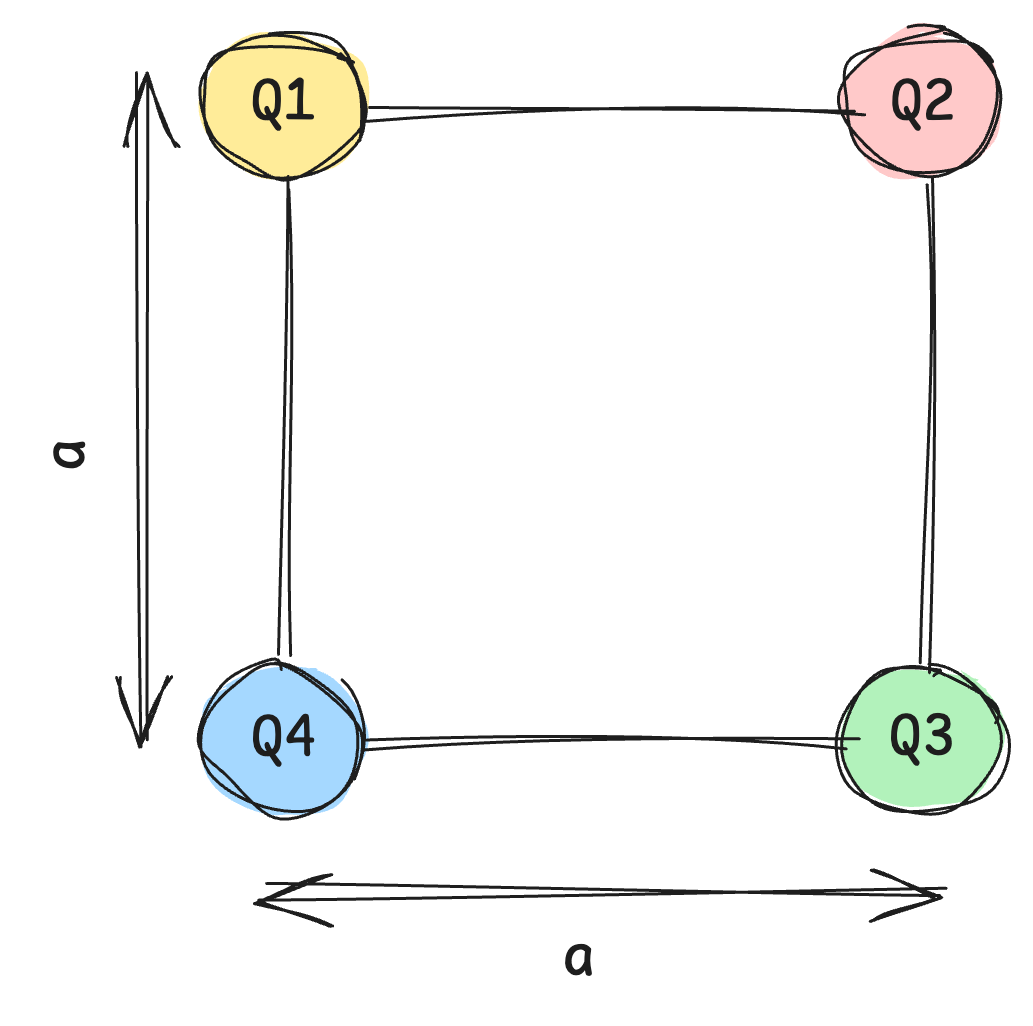
\includegraphics[width=0.3\textwidth]{figures/Q7.png}
\end{figure}
To solve this problem, one has to split into x and y components: 
$$D = \sqrt{(0.025\text{m})^2 + (0.025\text{m})^2}$$
$$E_x = \frac{1}{4 \pi\epsilon_0 D^2} \cos 45 \left(10 \text{nC} - 20 \text{nC} + 20 \text{nC} - 10 \text{nC} \right) = 0$$
$$E_y = \frac{1}{4 \pi\epsilon_0 D^2} \sin 45 \left(-10\text{nC} + 20 \text{nC} + 20 \text{nC} - 10 \text{nC}\right) = \frac{1}{4\pi\epsilon_0 D^2} \sin(45) 20 \times 10 ^{-9} C = \boxed{101730.65 \frac{\text{N}}{\text{C}}}$$


\end{document}